	\begin{figure}[H]
				\begin{center}
					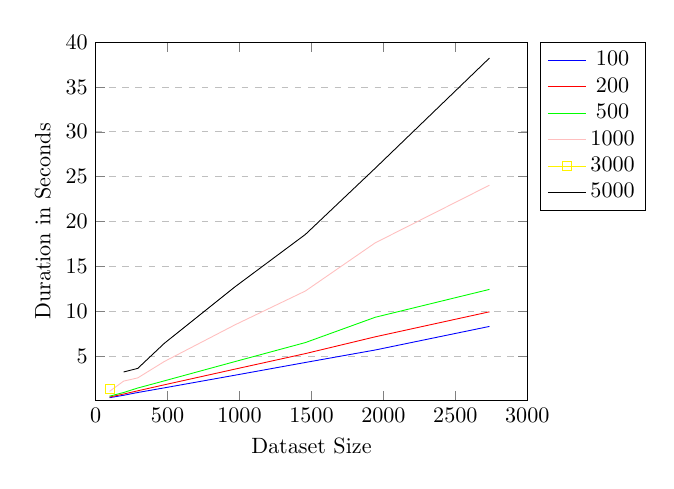
\begin{tikzpicture}[scale=0.8]
					\begin{axis}[
					/pgf/number format/.cd,
					use comma, 1000 sep={},
					xlabel={Dataset Size },
					ylabel={Duration in Seconds},
					xmin=0, xmax=3000,
					ymin=0, ymax=40,
					xtick={0,500,1000,1500,2000,2500,3000},
					ytick={5,10,15,20,25,30,35,40},
					legend pos=outer north east,
					ymajorgrids=true,
					grid style=dashed,
					]
					\addplot[color=blue,mark=no,]
					coordinates {
						(97,0.35)(195,0.62)(293,0.93)(478,1.45)(969,2.86)(1458,4.28)(1943,5.67)(2737,8.30)
					};
					\addplot[color=red,mark=no,]
					coordinates {
						(97,0.42)(195,0.76)(293,1.12)(478,1.79)(969,3.54)(1458,5.27)(1943,7.14)(2737,9.93)
					};
					\addplot[color=green,mark=no,]
					coordinates {
						(97,0.52)(195,0.93)(293,1.43)(478,2.23)(969,4.38)(1458,6.50)(1943,9.32)(2737,12.43)
					};
					\addplot[color=pink,mark=no,]
					coordinates {
						(97,1.06)(195,2.20)(293,2.56)(478,4.39)(969,8.48)(1458,12.25)(1943,17.62)(2737,24.05)	
					};
					\addplot[color=yellow,mark=square,]
					coordinates {
						(97,1.36)
					};
					\addplot[color=black,mark=no,]
					coordinates {
						(195,3.22)(293,3.62)(478,6.42)(969,12.72)(1458,18.56)(1943,25.94)(2737,38.23)
					};	
					\legend{100,200,500,1000,3000,5000}					
					\end{axis}
					\end{tikzpicture}
					\captionsetup{width=0.8\textwidth}
					\caption[Training Duration]{Training Duration as Function of Set Size and Number of Features with the Bag-of-Words Approach}
					\label{fig:duration_growth}
				\end{center}
			\end{figure} 